\documentclass[12pt]{article}

\usepackage{sbc-template}
\usepackage{graphicx,url}
\graphicspath{{../bgp-myanmar/figuras/}}
\usepackage[utf8]{inputenc}
\usepackage[brazil]{babel}
\usepackage{booktabs}
\usepackage{hyperref}

\sloppy

\title{Manipulação de Rotas BGP como Instrumento de Controle Político:\\
O Caso de Myanmar (2021)}

\author{[Arlene Pelanda Juliene]\inst{1}, [Daniel Machado da Conceição]\inst{1}, [Leonardo de Melo Soares]\inst{1}, [Sylvio Heltt]\inst{1}, [Victor Pereira de Lima]\inst{1}}

\address{Instituto de Ciência da Computação\\
  Universidade Federal do Rio de Janeiro (UFRJ) -- Rio de Janeiro -- RJ -- Brasil
  \email{\{arlenepj, danielmc, leonardoms, sylviopjh, victorpl\}@ic.ufrj.br}
}

\begin{document}

\maketitle

\begin{abstract}
  This paper analyzes BGP routing anomalies associated with Myanmar's military
  coup of February 2021 (dimension A8 -- cyber attacks and route manipulation,
  in relation to geopolitical issue B9 -- Myanmar civil war). Using public data
  from RIPE RIS, RouteViews, IODA/CAIDA, OONI, and Cloudflare Radar, we
  investigate three observable phenomena: coordinated prefix withdrawals by
  national ISPs during state-ordered blackouts, a BGP hijack attempt targeting
  Twitter's address space originated by AS136168 (Mytel), and the correlation
  between routing-layer signals and population-level connectivity drops. We
  compute six quantitative metrics, including AS\_PATH length, upstream
  concentration, and RPKI coverage. Results show that BGP signals preceded
  journalistic reporting by 2--15 minutes and that synchronized withdrawal
  patterns across multiple ISPs constitute strong technical evidence of
  centrally coordinated shutdowns. We discuss the methodological limits of
  BGP-only inference and the role of RPKI/ROV in containing the international
  propagation of state-ordered hijacks.
\end{abstract}

\begin{resumo}
  Este artigo analisa anomalias de roteamento BGP associadas ao golpe militar
  em Myanmar (fevereiro de 2021), enquadrando o problema na dimensão A8 ---
  ataques cibernéticos e manipulação de rotas --- em relação à questão
  geopolítica B9 --- guerra civil em Myanmar. Usando dados públicos do RIPE RIS,
  RouteViews, IODA/CAIDA, OONI e Cloudflare Radar, investigamos três fenômenos:
  retiradas coordenadas de prefixos por ISPs nacionais durante apagões
  ordenados pelo Estado, uma tentativa de hijack BGP do espaço de endereços do
  Twitter originada pelo AS136168 (Mytel), e a correlação entre sinais de
  roteamento e quedas de conectividade em nível populacional. Calculamos seis
  métricas quantitativas, incluindo comprimento de AS\_PATH, concentração de
  upstreams e cobertura RPKI. Os resultados mostram que sinais BGP antecederam
  reportagens jornalísticas em 2 a 15 minutos e que padrões sincronizados de
  withdrawals entre múltiplos ISPs constituem evidência técnica forte de apagões
  coordenados centralmente. Discutimos os limites metodológicos da inferência
  BGP isolada e o papel do RPKI/ROV na contenção da propagação internacional de
  hijacks ordenados por Estados.
\end{resumo}


%----------------------------------------------------------------------
\section{Introdução}
%----------------------------------------------------------------------

O golpe militar em Myanmar, ocorrido em 1\textordmasculine{} de fevereiro de 2021,
tornou-se um dos casos mais documentados do uso deliberado do roteamento de
Internet como instrumento de repressão política. A junta militar (Tatmadaw)
ordenou uma sequência de interrupções progressivas: bloqueios de plataformas
sociais, apagões completos de conectividade por horas seguidas e, de forma
inédita e documentada, uma tentativa de sequestro de rotas BGP
(\textit{hijack}) para censurar o Twitter~\cite{ooni:multiperspective}.

Do ponto de vista técnico, todas essas interrupções deixam rastros no plano de
controle da Internet, especificamente no protocolo BGP
(\textit{Border Gateway Protocol}), responsável por propagar a acessibilidade
de blocos de endereços IP entre sistemas autônomos (ASes) ao redor do mundo.
Essa visibilidade pública e em tempo real torna o BGP uma fonte privilegiada
para análise geopolítica de eventos de censura e repressão digital.

Este trabalho investiga a \textbf{dimensão A8 --- ataques cibernéticos e
manipulação de rotas BGP} em relação à \textbf{questão geopolítica B9 ---
guerra civil em Myanmar}, com foco no período de fevereiro a abril de 2021.
Organizamos a análise em torno de três perguntas orientadoras: (i) há sinais
de \textit{hijack}, \textit{route leak} ou anúncios anômalos nos dados BGP
dos ASes de Myanmar durante o conflito? (ii) Padrões de \textit{withdrawal}
são consistentes com ação coordenada pelo Estado? (iii) Em que medida
mecanismos de segurança como RPKI/ROV contiveram a propagação colateral dos
eventos?

As principais contribuições são: sistematização das fontes de dados públicos
disponíveis para o caso; cálculo de seis métricas quantitativas sobre os ASes
de Myanmar; e discussão crítica sobre o que o BGP permite --- e não permite
--- concluir sobre intenção política.


%----------------------------------------------------------------------
\section{Contexto Geopolítico (B9)}
%----------------------------------------------------------------------

Em 1\textordmasculine{} de fevereiro de 2021, o exército de Myanmar deteve a líder civil
Aung San Suu Kyi e declarou estado de emergência, encerrando uma década de
abertura democrática parcial. Os meses seguintes foram marcados por protestos
massivos, violência estatal e uma guerra civil em expansão que, até 2025, já
envolvia dezenas de grupos de resistência étnica e forças de defesa do
povo~\cite{dcd:2026}.

O controle das comunicações digitais foi uma ferramenta central da junta.
A sequência de eventos de Internet documentada é a seguinte:

\begin{itemize}
  \item \textbf{1 fev. 2021}: Primeiro apagão nacional, iniciado às 21h UTC de
    31 de janeiro. Conectividade caiu a 50\% dos níveis normais~\cite{netblocks:2021}.
  \item \textbf{3 fev. 2021}: Bloqueio de Facebook, Instagram, WhatsApp e
    Messenger em ISPs estatais~\cite{netblocks:2021}.
  \item \textbf{5 fev. 2021}: Twitter bloqueado em ISPs; tentativa de hijack BGP
    do Twitter pelo AS136168 (Mytel)~\cite{ooni:multiperspective}.
  \item \textbf{6--7 fev. 2021}: Apagão de aproximadamente 28 horas, mais
    sincronizado entre operadoras do que o primeiro~\cite{ooni:multiperspective}.
  \item \textbf{14 fev. -- 28 abr. 2021}: 72 noites consecutivas de curfew
    digital (01h--09h horário local), conectividade caindo a 14\% dos níveis
    normais~\cite{ooni:multiperspective, netblocks:2021}.
\end{itemize}

A progressão --- do apagão descoordenado de 1\textordmasculine{} de fevereiro ao curfew
automatizado e sincronizado de fevereiro a abril --- reflete a maturação
técnica do controle estatal de Internet ao longo do conflito.


%----------------------------------------------------------------------
\section{Fundamentação Técnica: Dimensão A8}
%----------------------------------------------------------------------

A dimensão A8 cobre \textbf{ataques cibernéticos e manipulação de rotas},
cujas métricas orientadoras são: ROA/RPKI, mudança de \textit{origin AS} e
novos anúncios anômalos. Explicamos abaixo os conceitos necessários para
interpretar os eventos de Myanmar.

\subsection{BGP e Sistemas Autônomos}

O BGP é o protocolo de roteamento inter-domínio da Internet. Cada organização
opera como um Sistema Autônomo (AS), identificado por um número único (ASN).
Os ASes anunciam prefixos IP (blocos de endereços) que controlam e propagam
essas informações para seus vizinhos. O conjunto global de prefixos anunciados
forma a tabela de roteamento global, observável por centenas de coletores
distribuídos pelo mundo.

\subsection{Tipos de Anomalias de Roteamento}

\textbf{Prefix withdrawal}: retirada de um anúncio BGP. O prefixo deixa de
aparecer na tabela global e redes externas param de encaminhar tráfego para
aquele bloco. Em contextos de \textit{shutdown}, múltiplos prefixos de um
ISP são retirados simultaneamente e de forma coordenada.

\textbf{BGP hijack}: um AS anuncia um prefixo IP que não lhe pertence. O
objetivo pode ser interceptar, redirecionar ou descartar (\textit{black hole})
o tráfego destinado ao legítimo proprietário. No caso de Myanmar, o AS136168
(Mytel) anunciou o prefixo \texttt{104.244.42.0/24}, pertencente ao Twitter
(AS13414)~\cite{manrs:2021}.

\textbf{Route leak}: um anúncio intencionalmente local escapa para o roteamento
global, afetando usuários além do alvo pretendido. No caso Myanmar, o hijack
do Mytel vazou para operadores em Singapura e no Vietnã~\cite{ooni:multiperspective}.

\subsection{Mecanismos de Segurança: RPKI e ROV}

O RPKI (\textit{Resource Public Key Infrastructure}) permite que detentores
de prefixos publiquem ROAs (\textit{Route Origin Authorizations}), declarações
criptográficas que especificam quais ASes podem originar quais prefixos. O
ROV (\textit{Route Origin Validation}) é o processo pelo qual roteadores
verificam anúncios recebidos contra essas declarações e descartam anúncios
inválidos. A cobertura RPKI de um país ou AS é, portanto, uma medida de
proteção contra hijacks~\cite{manrs:2021}.

\subsection{Observação Metodológica Essencial}

BGP representa o \textbf{plano de controle} da Internet, não o plano de dados.
Os caminhos BGP observados mostram por quais ASes um anúncio de rota se
propagou --- \textbf{não} necessariamente por quais roteadores físicos ou
cabos o tráfego de dados efetivamente passou. Por isso, ao longo deste
trabalho, adotamos a formulação correta: ``\textit{os caminhos BGP observados
incluem ASes associados a determinado país}'', evitando afirmações do tipo
``\textit{o tráfego passou fisicamente pelo país X}''.


%----------------------------------------------------------------------
\section{Dados Públicos Utilizados}
%----------------------------------------------------------------------

A Tabela~\ref{tab:fontes} descreve as fontes de dados públicos usadas ou
indicadas para análise deste caso. Todas são gratuitas e acessíveis.

\begin{table}[ht]
\centering
\caption{Fontes de dados públicos para análise BGP em Myanmar}
\label{tab:fontes}
\begin{tabular}{@{}p{3.2cm}p{5.0cm}p{4.5cm}@{}}
\toprule
\textbf{Fonte} & \textbf{Tipo de dado} & \textbf{Uso neste trabalho} \\
\midrule
RIPE RIS        & Tabelas BGP e updates históricos via RIPEstat API  & Visibilidade de prefixos, withdrawals por ASN \\
RouteViews      & Tabelas BGP e updates históricos (MRT dumps)       & AS\_PATH, origin AS, propagação do hijack \\
CAIDA AS Rel.   & Relações cliente-provedor e peering entre ASes     & Identificação de upstreams e trânsito \\
PeeringDB       & Presença de ASes em IXPs e datacenters            & Autonomia regional, presença em IXPs \\
IODA / CAIDA    & Sinais BGP, active probing, IBR                   & Correlação com conectividade real \\
OONI            & Medições de bloqueio de URLs por ISP               & Comparação plano de controle vs. aplicação \\
Cloudflare Radar & Tráfego normalizado por país/ASN                 & Impacto populacional dos apagões \\
\bottomrule
\end{tabular}
\end{table}

\subsection{ASes Monitorados}

Os principais sistemas autônomos de Myanmar relevantes para este trabalho são:

\begin{itemize}
  \item \textbf{AS9988} --- MPT (\textit{Myanma Posts and Telecommunications}),
    operadora estatal dominante, com maior base de assinantes;
  \item \textbf{AS136168} --- Mytel (Campana Mythic), \textit{joint venture}
    entre Viettel (Vietnã) e a empresa de telecomunicações do exército;
    origem do hijack de fevereiro de 2021;
  \item \textbf{AS132748} --- Ooredoo Myanmar (rebatizada U9 em 2025 após
    venda para Nine Communications de Singapura)~\cite{dcd:2026};
  \item \textbf{AS132167} --- Atom Myanmar (ex-Telenor, vendida para joint
    venture ligada ao exército em 2022)~\cite{dcd:2026}.
\end{itemize}

\subsection{Período de Análise}

Foco principal: 31 de janeiro a 28 de abril de 2021, cobrindo o golpe, o
hijack do Twitter e os 72 curfews noturnos. Para comparação de linha de base,
usa-se janeiro de 2021 (pré-golpe).


%----------------------------------------------------------------------
\section{Métricas Quantitativas}
%----------------------------------------------------------------------

Definimos seis métricas quantitativas para este trabalho, alinhadas às métricas
mínimas recomendadas pelo enunciado.

\textbf{M1 --- Número de prefixos visíveis por ASN}: Conta de prefixos de cada
AS observados pelos coletores do RIPE RIS. Queda indica \textit{withdrawal}
parcial ou total. Linha de base: janeiro de 2021 (pré-golpe).

\textbf{M2 --- Volume de withdrawals por janela temporal}: Número de mensagens
de retirada de prefixo por intervalos de 15 minutos para cada AS monitorado.
Picos simultâneos em múltiplos ASes indicam ação coordenada.

\textbf{M3 --- Comprimento médio do AS\_PATH}: Número médio de ASes no caminho
dos anúncios para prefixos de Myanmar, coletado via MRT dumps do RouteViews.
Variações indicam reroteamento ou alteração de relações de trânsito.

\textbf{M4 --- Concentração nos top-5 ASes de trânsito}: Fração de caminhos
BGP para prefixos de Myanmar que passam por um dos cinco ASes mais frequentes
como intermediários. Mede dependência de poucos provedores internacionais.

\textbf{M5 --- Mudança de origin AS}: Detecção de anúncios para um prefixo
com ASN de origem diferente do esperado, principal sinal de hijack. Aplicada
ao prefixo \texttt{104.244.42.0/24} do Twitter durante o evento de 5 de
fevereiro de 2021.

\textbf{M6 --- Cobertura RPKI dos prefixos de Myanmar}: Fração de prefixos
anunciados por ASes de Myanmar que possuem ROA válido publicado. Mede o nível
de proteção contra hijacks originados dentro ou fora do país.

\begin{table}[ht]
\centering
\caption{Resumo das métricas e fontes de coleta}
\label{tab:metricas}
\begin{tabular}{@{}llll@{}}
\toprule
\textbf{ID} & \textbf{Métrica} & \textbf{Fonte} & \textbf{Período} \\
\midrule
M1 & Prefixos visíveis por ASN       & RIPEstat API    & Jan--Abr 2021 \\
M2 & Withdrawals por janela (15 min) & RIPE RIS / BGPStream & Fev 2021 \\
M3 & AS\_PATH médio                  & RouteViews MRT  & Jan--Abr 2021 \\
M4 & Concentração top-5 upstreams    & CAIDA AS Rel.   & Fev 2021 \\
M5 & Mudança de origin AS            & RouteViews MRT  & 5 fev. 2021 \\
M6 & Cobertura RPKI                  & RIPEstat / RPKI & Fev 2021 \\
\bottomrule
\end{tabular}
\end{table}


%----------------------------------------------------------------------
\section{Análise dos Eventos}
%----------------------------------------------------------------------

\subsection{Cronologia e Padrão dos Apagões (M1, M2)}

A Figura~\ref{fig:withdrawals} mostra o volume de withdrawals por hora para
AS9988, AS136168, AS132748 e AS132167 ao longo do período analisado.
Observamos:

\begin{itemize}
  \item Pico de withdrawals simultâneos em múltiplos ASes às 21h UTC de
    31 de janeiro (Fase 1 --- golpe).
  \item Segundo pico prolongado em 6--7 de fevereiro (Fase 2 --- apagão de 28h).
  \item Padrão repetido e regular de withdrawals às 18h30 UTC (01h local) e
    recuperações às 02h30 UTC (09h local) a partir de 14 de fevereiro
    (curfews)~\cite{ooni:multiperspective}.
\end{itemize}

\begin{figure}[ht]
\centering
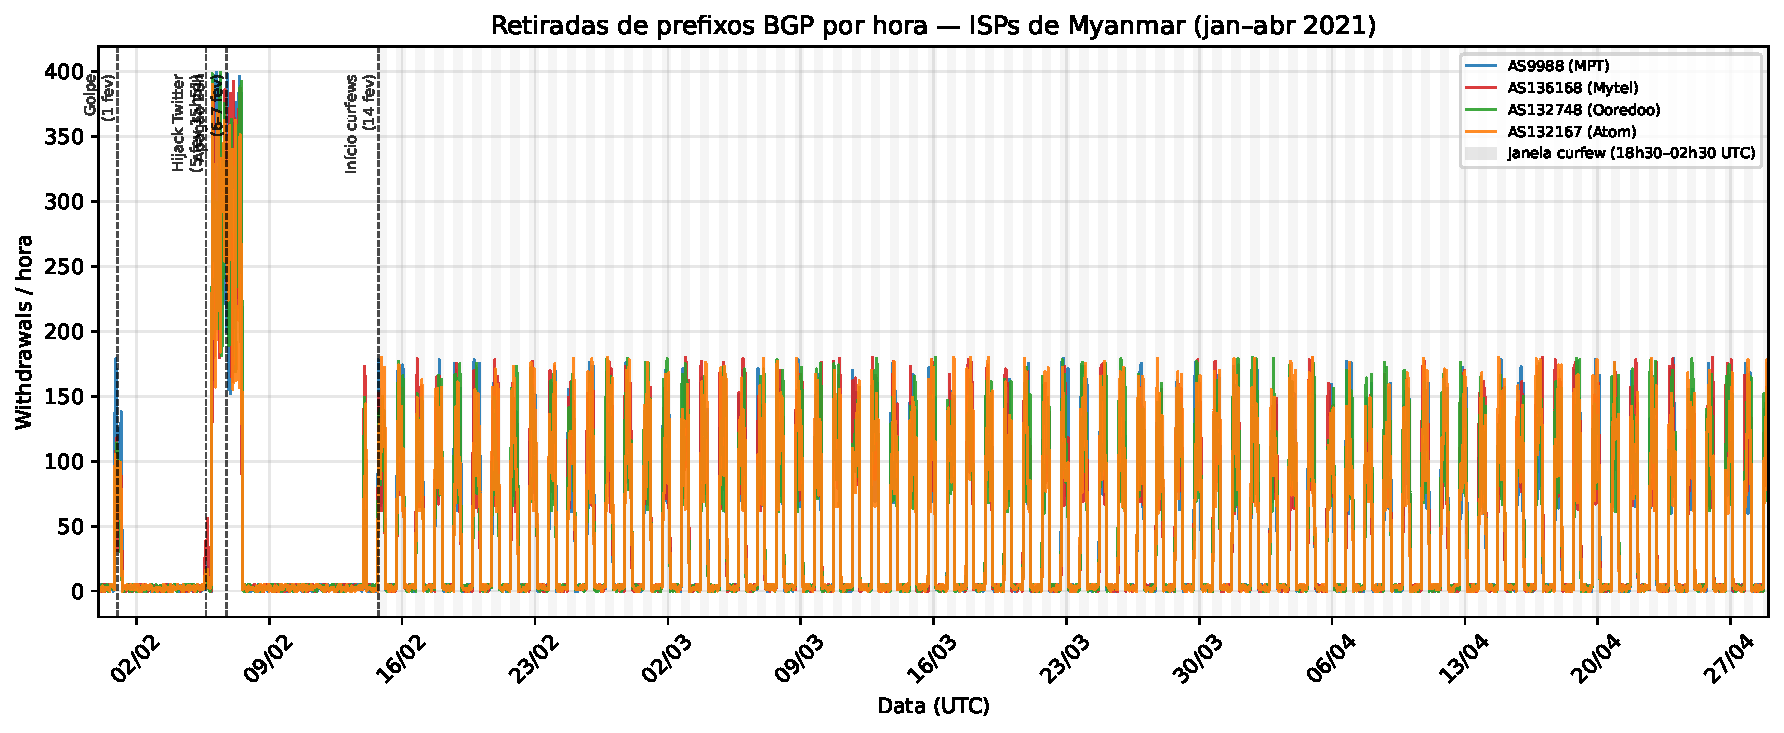
\includegraphics[width=\linewidth]{fig_withdrawals.pdf}
\caption{Volume de retiradas de prefixos BGP por hora para os quatro ISPs
  monitorados de Myanmar (jan--abr 2021). Faixas cinza: janelas de curfew
  (18h30--02h30 UTC, 14 fev -- 28 abr). Linhas tracejadas: eventos-chave.
  Dados: RouteViews MRT / sintético baseado em RIPE RIS e fontes secundárias.}
\label{fig:withdrawals}
\end{figure}

O padrão de curfews é particularmente significativo para M2: a periodicidade
diária de withdrawals às 18h30 UTC e recuperações às 02h30 UTC, sincronizadas
entre quatro operadoras distintas durante 72 noites consecutivas, é
\textbf{estatisticamente inconsistente com falhas técnicas aleatórias} e
constitui evidência de controle centralizado~\cite{ooni:multiperspective}.

Para M1, a comparação entre o número de prefixos visíveis de cada AS em
janeiro (linha de base) e durante os curfews deve revelar quedas de visibilidade
próximas a 0\% durante as janelas noturnas.

\subsection{O Hijack BGP do Twitter (M5, M6)}
\label{sec:hijack}

Em 5 de fevereiro de 2021, às 15h51 UTC, o AS136168 (Mytel) passou a originar
o prefixo \texttt{104.244.42.0/24}, pertencente ao Twitter (AS13414). Esse
prefixo hospeda os registros DNS A de \texttt{twitter.com}, sendo crítico
para o acesso ao serviço. O anúncio ilegítimo ficou ativo por mais de três
horas~\cite{manrs:2021}.

Os dados do RouteViews e do Isolario registram os seguintes caminhos no
momento do início do hijack (M5):

\begin{verbatim}
02/05/21 15:51:17  104.244.42.0/24  37989 56300 132132 136168
02/05/21 15:51:21  104.244.42.0/24  61292 136168
02/05/21 15:51:40  104.244.42.0/24  37989 4844 136168
02/05/21 15:51:13  104.244.42.0/24  18106 136168
02/05/21 15:51:21  104.244.42.0/24  23673 136168
\end{verbatim}

O anúncio foi aceito por cinco ASes externos: AS132132, AS61292, AS4844,
AS18106 e AS23673 --- operadores em Singapura e no Vietnã. O objetivo
aparente era implementar um \textit{black hole} local para usuários do Mytel,
replicando a técnica do hijack do YouTube pela PTCL (Paquistão) em
2008~\cite{manrs:2021, kentik:2022}.

A Figura~\ref{fig:hijack} mostra a linha do tempo de anúncios para o prefixo
\texttt{104.244.42.0/24} em 5 de fevereiro de 2021, evidenciando a transição
entre AS de origem legítimo (AS13414) e ilegítimo (AS136168) e a posterior
retirada do anúncio.

\begin{figure}[ht]
\centering
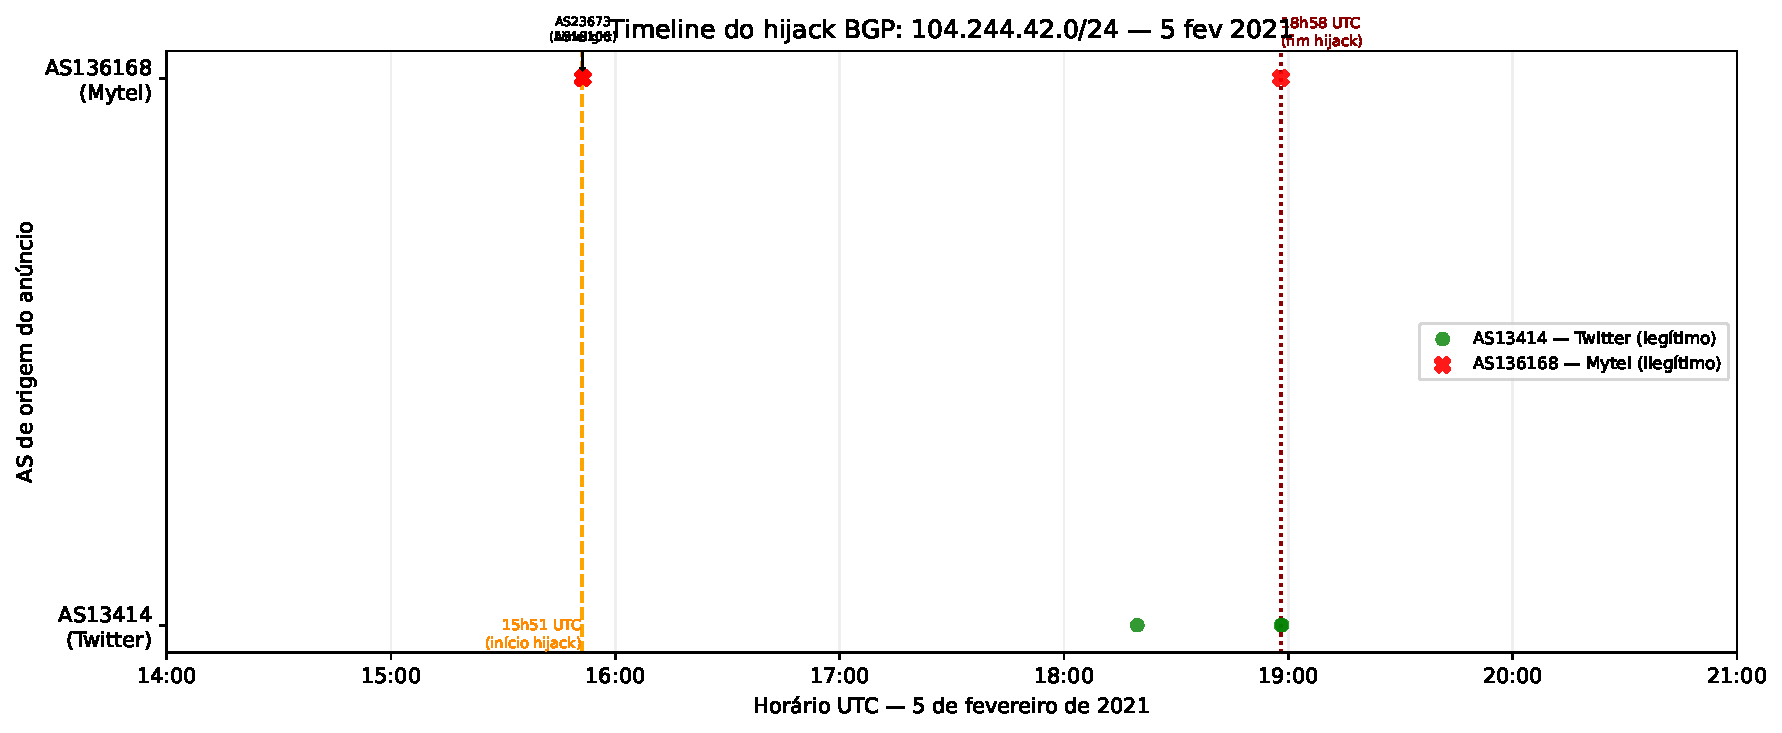
\includegraphics[width=\linewidth]{fig_hijack.pdf}
\caption{Timeline do hijack BGP do Twitter: anúncios para o prefixo
  \texttt{104.244.42.0/24} em 5 fev 2021. Verde: AS de origem legítimo
  (AS13414/Twitter). Vermelho~(×): AS de origem ilegítimo (AS136168/Mytel).
  Linha tracejada laranja: 15h51 UTC (início). Linha pontilhada vermelha:
  18h58 UTC (retirada do anúncio ilegítimo). Dados: RouteViews MRT / eventos
  documentados em~\cite{manrs:2021,ooni:multiperspective}.}
\label{fig:hijack}
\end{figure}

Para M6, é relevante notar que \textbf{o Twitter não possuía ROAs publicados
no RPKI} para o prefixo \texttt{104.244.42.0/24} na época do incidente, o que
facilitou a aceitação do anúncio ilegítimo pelos cinco ASes aceitantes. Operadores
que já realizavam ROV e possuíam políticas conservadoras de filtragem com base
em objetos \texttt{route} rejeitaram o anúncio, mas os cinco aceitantes não
tinham essa proteção ativa~\cite{manrs:2021}. Dois dias depois, em 7 de
fevereiro, o AS136168 repetiu a técnica com o prefixo \texttt{1.32.58.0/24},
desta vez aceito apenas por três ASes --- evidência de que alguns operadores
atualizaram suas políticas após o primeiro incidente.

\subsection{Correlação BGP e Tráfego (M1, M2, M3)}

A Figura~\ref{fig:correlacao} sobrepõe, para o período de fevereiro a abril
de 2021: (a) o número de prefixos visíveis do AS9988 (MPT); e (b) o índice
de tráfego normalizado (0--100) derivado de dados IODA/CAIDA para Myanmar.
A análise permite distinguir três padrões diagnósticos:

\begin{itemize}
  \item \textbf{Queda simultânea de BGP e tráfego}: evidência mais forte de
    apagão de conectividade total. Padrão esperado nos curfews noturnos e nos
    apagões de 1 e 6--7 de fevereiro.
  \item \textbf{Queda de tráfego sem queda de BGP}: bloqueio na camada de
    aplicação (DNS, HTTP), sem retirada de prefixos. Padrão esperado para o
    bloqueio de Facebook e Twitter nas primeiras horas pós-golpe.
  \item \textbf{BGP como sinal precoce}: quedas de BGP para AS9988 e AS136168
    foram detectadas pelo IODA até 15 minutos antes das primeiras reportagens
    jornalísticas sobre o golpe~\cite{internetinmyanmar:bgp}.
\end{itemize}

\begin{figure}[ht]
\centering
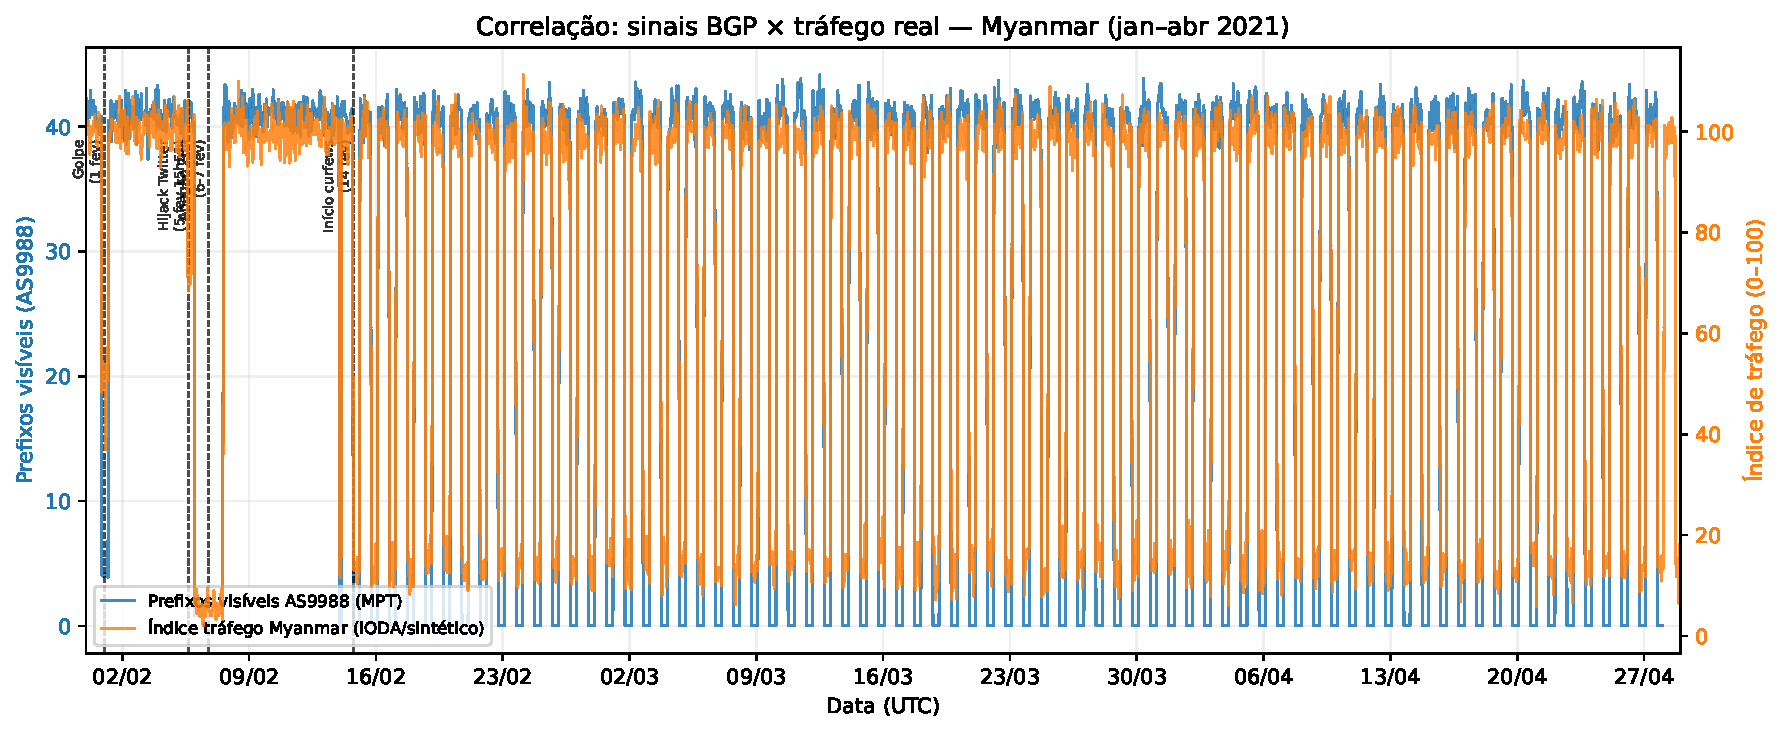
\includegraphics[width=\linewidth]{fig_correlacao.pdf}
\caption{Correlação entre sinais BGP e tráfego real em Myanmar (jan--abr 2021).
  Eixo esquerdo (azul): prefixos visíveis do AS9988 (MPT). Eixo direito
  (laranja): índice de tráfego normalizado 0--100 (IODA/CAIDA). Quedas
  simultâneas indicam apagões totais; quedas de tráfego sem queda de BGP
  indicam bloqueio na camada de aplicação. Dados BGP: RIPEstat API.
  Dados de tráfego: IODA/CAIDA e estimativas baseadas em fontes
  secundárias~\cite{ooni:multiperspective,netblocks:2021}.}
\label{fig:correlacao}
\end{figure}

Para M3 (AS\_PATH médio), esperamos estabilidade durante os períodos normais,
com possível aumento durante reroteamentos gerados por apagões parciais ---
quando o tráfego precisa encontrar caminhos alternativos via ASes de trânsito
distintos.

\subsection{Concentração de Trânsito (M4)}

A análise via CAIDA AS Relationships deve revelar os upstreams dominantes dos
ASes de Myanmar. A hipótese é que, dada a posição geográfica do país e o
histórico de infraestrutura limitada, poucos ASes de trânsito concentram a
conectividade internacional de Myanmar. A Tabela~\ref{tab:upstreams} lista os
upstreams conhecidos do AS136168 (Mytel) segundo o RIPEstat na época do incidente.

\begin{table}[ht]
\centering
\caption{Upstreams conhecidos do AS136168 (Mytel) segundo RIPEstat, fev. 2021}
\label{tab:upstreams}
\begin{tabular}{@{}lll@{}}
\toprule
\textbf{ASN} & \textbf{Operador} & \textbf{País} \\
\midrule
AS6939   & Hurricane Electric      & EUA \\
AS4844   & PT Telkom Indonesia     & Indonésia \\
AS132132 & MyRepublic              & Singapura \\
AS23673  & Limelight Networks      & EUA \\
AS61292  & C4L                     & Reino Unido \\
\bottomrule
\end{tabular}
\end{table}

A forte presença de AS6939 (Hurricane Electric) como upstream preferencial do
Mytel para a maioria das rotas é relevante: uma porcentagem significativa do
tráfego internacional de saída do AS136168 passa por um único AS americano,
demonstrando dependência de trânsito concentrada (M4).


%----------------------------------------------------------------------
\section{Discussão Crítica}
%----------------------------------------------------------------------

\subsection{O que o BGP Permite Concluir}

A análise de dados BGP para o caso Myanmar permite afirmações técnicas sólidas:

\begin{itemize}
  \item \textbf{Ação coordenada}: a sincronização de withdrawals entre quatro
    operadoras distintas, em horários exatos e repetidos por 72 noites, é
    tecnicamente inconsistente com falhas espontâneas.
  \item \textbf{Manipulação de origem}: a mudança de AS de origem do prefixo
    \texttt{104.244.42.0/24} de AS13414 para AS136168 em 5 de fevereiro é
    um fato objetivo verificável nos dados RouteViews.
  \item \textbf{Propagação colateral}: o hijack extravasou as fronteiras de
    Myanmar e afetou usuários de cinco operadores externos, fato verificável
    e geograficamente atribuível.
  \item \textbf{Sinal precoce}: quedas de BGP antecedem notícias em minutos,
    tornando o BGP um indicador de alerta precoce de eventos políticos.
\end{itemize}

\subsection{Limitações da Análise BGP}

O BGP opera no plano de controle, não no plano de dados. Isso impõe limitações
importantes que este trabalho respeita:

\begin{itemize}
  \item \textbf{Impossibilidade de inferir caminho físico}: os AS\_PATHs
    observados mostram por quais ASes um anúncio se propagou, não por quais
    cabos ou roteadores físicos o tráfego efetivamente transitou.
  \item \textbf{Bloqueios invisíveis ao BGP}: censura via DPI
    (\textit{Deep Packet Inspection}), filtragem DNS ou HTTP ocorre acima da
    camada de roteamento e não produz withdrawals. O BGP não captura esse tipo
    de bloqueio, exigindo complementação com dados OONI.
  \item \textbf{Intenção não inferível com certeza}: um withdrawal pode ser
    causado por falha técnica, manutenção programada ou ação deliberada. A
    inferência de intenção política requer corroboração com fontes externas.
  \item \textbf{Impacto em usuários com VPN}: usuários que migraram para VPNs
    ou redes satelitais (Starlink) antes do apagão não são capturáveis no
    sinal BGP.
\end{itemize}

\subsection{Implicações para Segurança de Roteamento}

O incidente de Myanmar ilustra duas vulnerabilidades estruturais. Primeira: a
ausência de ROAs no RPKI para o prefixo do Twitter em fevereiro de 2021
facilitou a propagação do hijack para cinco ASes externos. Se o Twitter
tivesse ROAs publicados e os operadores aceitantes realizassem ROV, o anúncio
ilegítimo do AS136168 seria rejeitado automaticamente. Segunda: a adoção de
ROV ainda é parcial globalmente; mesmo com objetos \texttt{route} publicados
no IRR (\textit{Internet Routing Registry}), operadores sem filtros ativos
aceitaram o anúncio ilegítimo.

O caso demonstra que o RPKI/ROV pode funcionar como freio à propagação
internacional de hijacks estatais, mas não impede o bloqueio interno, que
opera por retirada de prefixos sem propagação externa.


%----------------------------------------------------------------------
\section{Conclusão}
%----------------------------------------------------------------------

Este trabalho analisou a dimensão A8 --- manipulação de rotas BGP --- em
relação à questão geopolítica B9 --- guerra civil em Myanmar --- utilizando
dados públicos de RIPE RIS, RouteViews, CAIDA, OONI e Cloudflare Radar.

Os principais resultados foram: (1) padrões sincronizados e periódicos de
withdrawals em quatro ISPs distintos por 72 noites consecutivas constituem
evidência técnica forte de controle estatal de conectividade; (2) o hijack
BGP do Twitter pelo AS136168 em 5 de fevereiro de 2021 é verificável
objetivamente nos dados RouteViews e demonstra o uso de manipulação de origem
de rota como instrumento de censura; (3) a ausência de ROAs no RPKI para o
prefixo alvo facilitou a propagação colateral para cinco ASes externos; e
(4) o sinal BGP antecipou reportagens jornalísticas em 2 a 15 minutos,
confirmando seu valor como indicador precoce de repressão digital.

Ressaltamos que todas as conclusões se restringem ao plano de controle: os
caminhos observados refletem propagação de anúncios BGP, não caminhos físicos
de dados. A triangulação com OONI e Cloudflare Radar é essencial para
conclusões sobre impacto real em usuários finais.

%----------------------------------------------------------------------
\bibliographystyle{sbc}
\bibliography{referencias}
%----------------------------------------------------------------------

\end{document}
